
\documentclass[12pt,onecolumn]{article}
\usepackage[brazilian]{babel}
\usepackage[utf8]{inputenc}
\usepackage{graphicx}
\usepackage{caption}
\usepackage{subcaption}
\usepackage{float}
\usepackage{hyperref}
\usepackage{blindtext}

\begin{document}

\begin{titlepage}

	\title{
		\bf
		\LARGE Apostila de  \\
		\Huge  WordPress
	}

	\author{Gustavo Teixeira da Cunha Coelho \\ Henrique Gemignani Passos Lima}

	\maketitle

	\thispagestyle{empty}

	\vfill
	
	\center{Primeira Edição RC1}

\end{titlepage}

	\thispagestyle{empty}

\begin{center}
  Copyright (C) 2013 USPGameDev
\end{center}
\begin{figure}[ht]
  \centering
  
\includegraphics[width=\textwidth]{../CC-BY.png}
\end{figure}

\vfill

\begin{center}
A edição mais recente pode ser encontrada em:
\url{http://uspgamedev.org/apostilas/}
\end{center}

\vfill

Escrito por:
\begin{itemize}
  \item \textbf{Gustavo Teixeira da Cunha Coelho} \textit{(coelho at uspgamedev.org)}
  \item \textbf{Henrique Gemignani Passos Lima} \textit{(henrique at uspgamedev.org)}
\end{itemize}

% Page break.
\clearpage

% Print table of contents.
\tableofcontents

% Page break.
\clearpage

\section{Sobre o WordPress}
	O WordPress é um \href{http://pt.wikipedia.org/wiki/Sistema_de_gerenciamento_de_conte%C3%BAdo}{
	sistema de gerenciamento de contéudo} para Web, usado para a criação de blogs. Ele possui muitas 
	ferramentas que facilitam a criação do seu site e é o sistema de criação de blogs mais usado na internet.

	Para saber um pouco mais da história do WordPress  \href{http://wordpress.org/about/}{clique aqui}.
          
\section{Instalando}
	A instação do WordPress é responsabilidade de quem é o responsável por gerenciar o site em si 
	e não de quem apenas gerencia o conteúdo.

	Se você não tem um site, serviços como o \href{https://wordpress.com/}{WordPress.com} fornecem
	uma página com WordPress já instalado. Se for uma hospedagem comprada, consulte o CPanel ou similar
	se este possuiu uma instalação automática de WordPress.

\clearpage
\section{Postando}
	\subsection{Autorização}
		É importante notar que o WordPress possui um controle de acesso, logo 
		somente pessoas autorizadas podem criar novos posts.
		
		Para tal, precisamos realizar o login antes de podermos continuar com qualquer
		tarefa.
		\begin{figure}[H]
			\begin{subfigure}{.4\textwidth}
				\centering
				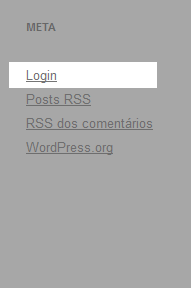
\includegraphics{login1.png}
				\caption{Link para a página de login}
			\end{subfigure}
			\begin{subfigure}{.4\textwidth}
				\centering
				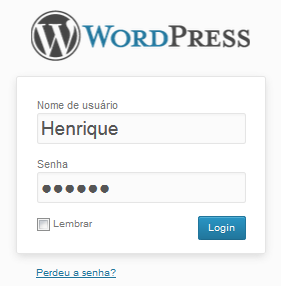
\includegraphics{login2.png}
				\caption{Digitando usuário e senha}
			\end{subfigure}
			\caption{Processo de login}
		\end{figure}
	
	
	\subsection{Criando um post}
		Criar um post é extremamente simples. O modo mais fácil de fazê-lo é usar a barra do WordPress,
		onde por padrão existe uma seção para criação de conteúdo novo, e clicar em Novo Post. Após isso
		basta usar o editor visual para gerar e publicar o post.
		\begin{figure}[H]
			\centering
			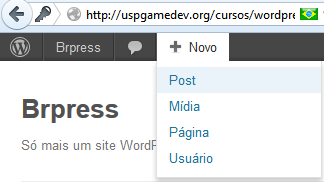
\includegraphics{post1.png}
			\caption{Usando a barra do WordPress}
		\end{figure}
		\begin{figure}[H]
			\centering
			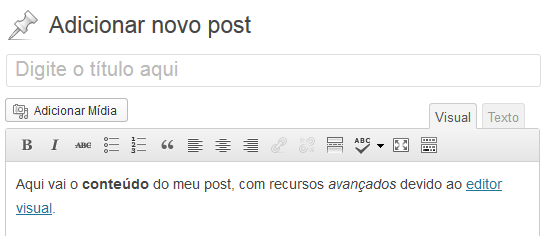
\includegraphics{post2.png}
			\caption{Usando o editor visual}
		\end{figure}
		\begin{figure}[H]
			\centering
			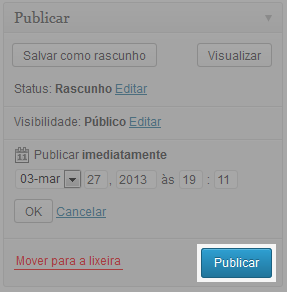
\includegraphics{post3.png}
			\caption{Publicando}
		\end{figure}

	\subsection{Categorias e Tags}
		Na hora de criação de um post, podemos adicionar categorias e tags 
		para agrupar posts quanto ao seu conteúdo. Como regra geral, as
		categorias são usadas para dizer sobre o que o post de uma maneira
		bastante abrangente. Já as tags são normalmente usadas para dizer
		mais especificamente sobre o conteúdo do post. Categorias e tags
		podem ser colocadas no momento de criação de um post, mas
		também podem ser colocadas após a crição de um post.
		\begin{figure}[H]
			\begin{subfigure}{.55\textwidth}
				\centering
				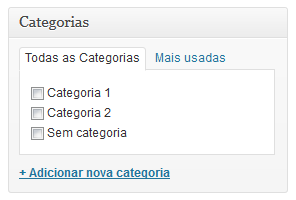
\includegraphics{categorias1.png}
				\caption{Adicinando categorias a um post}
			\end{subfigure}
			\begin{subfigure}{.4\textwidth}
				\centering
				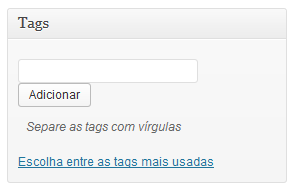
\includegraphics{tags1.png}
				\caption{Adicinando tags a um post}
			\end{subfigure}
		\end{figure}

	\subsection{Páginas}
		Um tipo especial de post no Wordpress são as Páginas.
		Essas páginas são tratadas de maneira especial pelo seu tema, como por
		exemplo listando todas na página inicial.
		\begin{figure}[H]
			\centering
			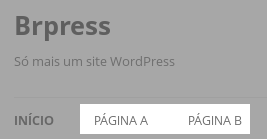
\includegraphics{page1.png}
			\caption{Lista de páginas do tema padrão}
		\end{figure}
		
\clearpage
\section{Conteúdo Elaborado}
	Não é apenas de texto que o blog vai ficar bom.
	\subsection{Imagens}
		Adicionar imagens no seu post é simples, basta clica em Adicionar Mídia.
		\begin{figure}[H]
			\centering
			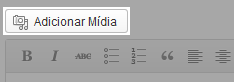
\includegraphics{midia1.png}
			\caption{Botão 'Adicionar Mídia'.}
		\end{figure}
		Feito isso, você pode ou enviar novas imagens para o site ou utilizar 
		aquelas que já estão disponíveis na aba Biblioteca de Mídia.
	\subsection{Vídeos}
		A forma mais fácil é enviar o vídeo para algum dos sites que o 
		\href{http://codex.wordpress.org/Embeds}{WordPress tem suporte} e 
		então colocar o link no post. O resto acontece sozinho.
		\begin{figure}[H]
			\centering
			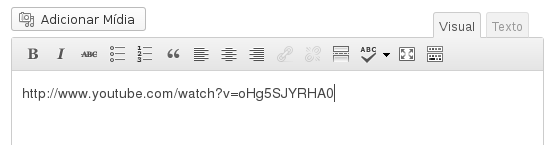
\includegraphics{video1.png}
			\caption{Colocando um link no post}
		\end{figure}
		\begin{figure}[H]
			\centering
			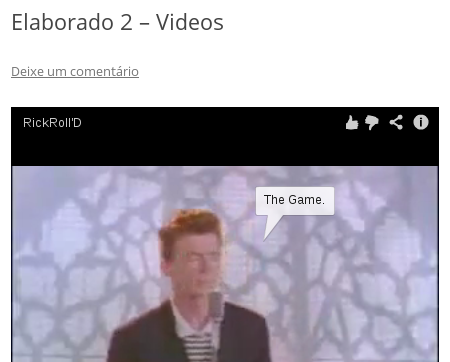
\includegraphics{video2.png}
			\caption{O video no post}
		\end{figure}
	\subsection{HTML}
		Todo post no WordPress na realidade é feito em HTML. O editor visual é uma
		forma de gerar esse HTML de uma forma simples e fácil e se mexer. A qualquer 
		momento você pode ir para o editor modo texto, ver e modificar o HTML gerado, 
		e então voltar ao edtior visual, com as modificações ativas.
		\begin{figure}[H]
			\centering
			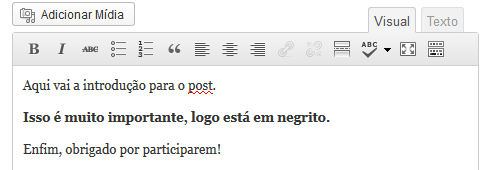
\includegraphics{html2.png}
			\caption{Post no modo visual.}
		\end{figure}
		\begin{figure}[H]
			\centering
			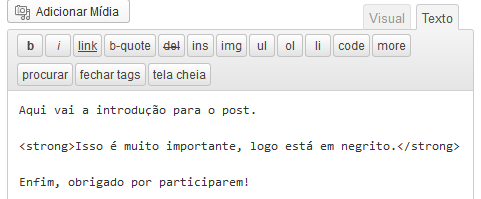
\includegraphics{html3.png}
			\caption{O mesmo post no modo texto.}
		\end{figure}
		\subsubsection{Adicionando um mapa do Google Maps}
			Como exemplo, aqui vai instruções de como colocar um mapa do Google Mapas
			no final do seu post.
			\begin{enumerate}
				\item Escreva o seu post normalmente, colocando tudo o que bem intender.
				\item Visite o Google Maps e ache o local de onde você quer colocar o mapa.
				\item Clique no botão de link e copie o texto no campo "Paste HTML to embed in website"
					\begin{figure}[H]
						\centering
						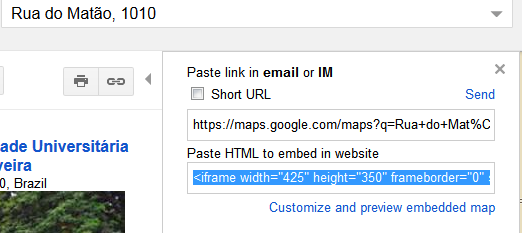
\includegraphics{html4.png}
						\caption{Pegando um bloco de HTML pronto.}
					\end{figure}
				\item Volte ao seu post, e mude para o editor de texto. Como queremos colocar
					o mapa no final, vá ate o fim e então cole o HTML que copiou do Google Maps.
				\item Pronto, você já pode voltar ao editor visual e encontrar um retangulo indicando que 
					existe algo excepcional ali, e que o editor visual não mostra.
				\item Clique em Visualizar, e veja o mapa dentro de seu post!
					\begin{figure}[H]
						\centering
						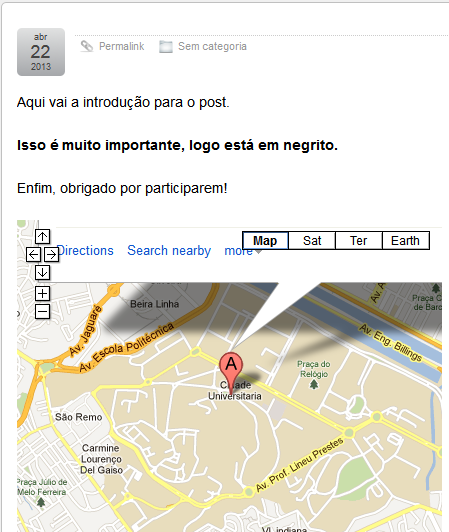
\includegraphics{html5.png}
						\caption{Visualizando o post com o módulo externo.}
					\end{figure}
			\end{enumerate}

\section{Temas}
	O tema padrão do WordPress é apenas uma das aparências que este pode ter. Embora
	seja possível alterar partes, como título, descrição, cores do texto e o fundo, para poder
	modificar além disso, é necessário trocar o \textit{tema} em si.
	
	%TODO: falar mais sobre temas! subsection sobre Suffision?
	
	\subsection{Gerenciando temas}
		\begin{figure}[H]
			\centering
			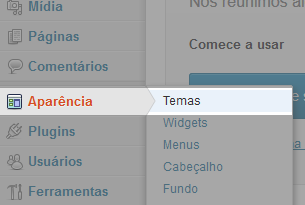
\includegraphics{tema1.png}
			\caption{Localizando a página de temas}
		\end{figure}
		Nesta página é possível personalizar o tema atual, adicionar menus, widgets
		ou mudar o tema ativo. Também é possível procurar temas novos para instalar.
		
\section{Widgets}
	\href{http://pt.wikipedia.org/wiki/Widget}{Widgets} podem ser adicionados ao seu site para 
	complementar as informações disponíveis aos seus usuários. Por padrão, novos sites WordPress
	já são criados com alguns Widgets, como um Widget para busca no seu site, um Widget mostrando 
	os Posts recentes, além de outros.
	\begin{figure}[H]
		\centering
		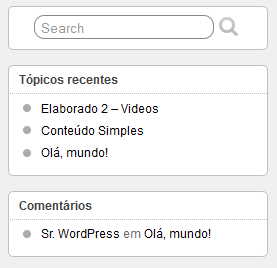
\includegraphics{widgets1.png}
		\caption{Exemplo de alguns Widgets padrões}
	\end{figure}

\end{document}
